
%(BEGIN_QUESTION)
% Copyright 2006, Tony R. Kuphaldt, released under the Creative Commons Attribution License (v 1.0)
% This means you may do almost anything with this work of mine, so long as you give me proper credit

Predict how the operation of this motor control circuit will be affected as a result of the following faults.  Consider each fault independently (i.e. one at a time, no coincidental faults):

$$\includegraphics[width=15.5cm]{i02321x01.eps}$$

\begin{itemize}
\item{} ``Stop'' pushbutton switch fails open:
\vskip 5pt
\item{} Relay contact CR1-1 fails open:
\vskip 5pt
\item{} Relay contact CR1-2 fails open:
\vskip 5pt
\item{} Relay coil CR1 fails open:
\end{itemize}

For each of these conditions, explain {\it why} the resulting effects will occur.

\vskip 20pt \vbox{\hrule \hbox{\strut \vrule{} {\bf Suggestions for Socratic discussion} \vrule} \hrule}

\begin{itemize}
\item{} Is this a single-phase motor or a three-phase motor?  How can you tell?
\item{} What would need to be changed in this circuit to reverse the rotation of the motor?
\item{} Suppose another technician suggests to you that the ``Run'' indicator lamp should be connected in parallel with the motor rather than in parallel with relay coil CR1.  Do you think this is a good idea?  Why or why not?
\item{} Modify this circuit to include a ``Jog'' pushbutton switch that runs the motor when pressed but immediately stops the motor when released (i.e. no ``latching'' function).
\end{itemize}

\underbar{file i02321}
%(END_QUESTION)





%(BEGIN_ANSWER)

\begin{itemize}
\item{} ``Stop'' pushbutton switch fails open: {\it Motor cannot start, lamp never energizes.}
\vskip 5pt
\item{} Relay contact CR1-1 fails open: {\it Motor starts and lamp energizes when ``Start'' button is pressed, but both immediately de-energize when it is released.}
\vskip 5pt
\item{} Relay contact CR1-2 fails open: {\it ``Motor run'' lamp turns on and off as expected, but the motor itself never runs.}
\vskip 5pt
\item{} Relay coil CR1 fails open: {\it Motor cannot start, but the lamp energizes when the ``Start'' pushbutton is pressed.}
\end{itemize}

%(END_ANSWER)





%(BEGIN_NOTES)

The purpose of this question is to approach the domain of circuit troubleshooting from a perspective of knowing what the fault is, rather than only knowing what the symptoms are.  Although this is not necessarily a realistic perspective, it helps students build the foundational knowledge necessary to diagnose a faulted circuit from empirical data.  Questions such as this should be followed (eventually) by other questions asking students to identify likely faults based on measurements.

\vskip 20pt \vbox{\hrule \hbox{\strut \vrule{} {\bf Virtual Troubleshooting} \vrule} \hrule}

This question is a good candidate for a ``Virtual Troubleshooting'' exercise.  Presenting the diagram to students, you first imagine in your own mind a particular fault in the system.  Then, you present one or more symptoms of that fault (something noticeable by an operator or other user of the system).  Students then propose various diagnostic tests to perform on this system to identify the nature and location of the fault, as though they were technicians trying to troubleshoot the problem.  Your job is to tell them what the result(s) would be for each of the proposed diagnostic tests, documenting those results where all the students can see.

During and after the exercise, it is good to ask students follow-up questions such as:

\begin{itemize}
\item{} What does the result of the last diagnostic test tell you about the fault?
\item{} Suppose the results of the last diagnostic test were different.  What then would that result tell you about the fault?
\item{} Is the last diagnostic test the best one we could do?
\item{} What would be the ideal order of tests, to diagnose the problem in as few steps as possible?
\end{itemize}

%INDEX% Relay, diagram: ladder logic

%(END_NOTES)


